\subsubsection{2.4. Kết quả kiểm thử trên mô hình CNN + MGAT + FastKAN/MLP với hai phương thức (hình ảnh và văn bản)}
\indent\indent Dưới đây là kết quả kiểm thử chi tiết của 12 mô hình CNN backbone + MGAT + FastKAN/MLP với hai phương thức (hình ảnh và văn bản), trong đó các giá trị được lấy từ lần chạy đạt kết quả cao nhất.\vspace{0.3cm}

%===================================================================
\textbf{* ResNet18 + MGAT + FastKAN/MLP:} 
\begin{table}[H]
\centering
\renewcommand{\arraystretch}{1.08}
\caption{\centering Classification report của FastKAN(1) và MLP(2) trên hai phương thức với backbone ResNet18}
\begin{tabular}{lccccccc}
\hline \textbf{Lớp} & \textbf{P(1)} & \textbf{R(1)} & \textbf{F1(1)} & \textbf{P(2)} & \textbf{R(2)} & \textbf{F1(2)} & \textbf{Support} \\ \hline

cho-noi-cai-rang
& 0.9130 & 0.9333 & \textbf{0.9231}
& 1.0000 & 0.7556 & 0.8608 & 45 \\

dua-bo-bay-nui
& 0.9783 & 1.0000 & \textbf{0.9890}
& 0.9574 & 1.0000 & 0.9783 & 45 \\

hoi-lim
& 0.9565 & 0.9778 & \textbf{0.9670}
& 0.9773 & 0.9556 & 0.9663 & 45 \\

le-hoi-nghinh-ong
& 0.8286 & 0.6444 & 0.7250
& 0.8333 & 0.7778 & \textbf{0.8046} & 45 \\

nghe-dan-tre
& 0.9783 & 1.0000 & \textbf{0.9890}
& 0.8654 & 1.0000 & 0.9278 & 45 \\

nghe-det-chieu
& 0.9778 & 0.9778 & \textbf{0.9778}
& 0.9512 & 0.8667 & 0.9070 & 45 \\

ok-om-bok
& 1.0000 & 0.9111 & \textbf{0.9535}
& 0.8400 & 0.9333 & 0.8842 & 45 \\

via-ba-chua-xu-nui-sam
& 0.7091 & 0.8667 & \textbf{0.7800}
& 0.8000 & 0.8889 & 0.8421 & 45 \\
\hline

\textbf{Accuracy}
& & & \textbf{0.9139}
& & & 0.8972 & 360 \\

\textbf{Macro avg}
& \textbf{0.9177} & \textbf{0.9139} & \textbf{0.9130}
& 0.9031 & 0.8972 & 0.8964 & 360 \\

\textbf{Weighted avg}
& \textbf{0.9177} & \textbf{0.9139} & \textbf{0.9130}
& 0.9031 & 0.8972 & 0.8964 & 360 \\
\hline
\end{tabular}
\end{table}

%===================================================================
\newpage
\textbf{* RegNetX400MF + MGAT + FastKAN/MLP:}
\begin{table}[H]
\centering
\renewcommand{\arraystretch}{1.08}
\caption{\centering Classification report của FastKAN(1) và MLP(2) trên hai phương thức với backbone RegNetX400MF}
\begin{tabular}{lccccccc}
\hline \textbf{Lớp} & \textbf{P(1)} & \textbf{R(1)} & \textbf{F1(1)} & \textbf{P(2)} & \textbf{R(2)} & \textbf{F1(2)} & \textbf{Support} \\ \hline

cho-noi-cai-rang
& 0.8600 & 0.9556 & 0.9053 
& 0.9149 & 0.9556 & \textbf{0.9348} & 45 \\

dua-bo-bay-nui 
& 0.9574 & 1.0000 & 0.9783 
& 0.9783 & 1.0000 & \textbf{0.9890} & 45 \\

hoi-lim 
& 0.8113 & 0.9556 & 0.8776 
& 0.9333 & 0.9333 & \textbf{0.9333} & 45 \\

le-hoi-nghinh-ong
& 0.7234 & 0.7556 & 0.7391 
& 0.7500 & 0.8000 & \textbf{0.7742} & 45 \\

nghe-dan-tre
& 1.0000 & 0.9778 & 0.9888 
& 0.9783 & 1.0000 & \textbf{0.9890} & 45 \\

nghe-det-chieu 
& 0.9487 & 0.8222 & 0.8810 
& 0.9556 & 0.9556 & \textbf{0.9556} & 45 \\

ok-om-bok 
& 0.9737 & 0.8222 & 0.8916 
& 0.9545 & 0.9333 & \textbf{0.9438} & 45 \\

via-ba-chua-xu-nui-sam 
& 0.7381 & 0.6889 & 0.7126 
& 0.8718 & 0.7556 & \textbf{0.8095} & 45 \\
\hline

\textbf{Accuracy}
& & & 0.8722
& & & \textbf{0.9167}  & 360 \\

\textbf{Macro avg} 
& 0.8766 & 0.8722 & 0.8718 
& \textbf{0.9171} & \textbf{0.9167} & \textbf{0.9162} & 360 \\

\textbf{Weighted avg}
& 0.8766 & 0.8722 & 0.8718 
& \textbf{0.9171} & \textbf{0.9167} & \textbf{0.9162} & 360 \\
\hline
\end{tabular}
\end{table}
%===================================================================
\textbf{* MobileNetV3 Large + MGAT + FastKAN/MLP:}
\begin{table}[H]
\centering
\renewcommand{\arraystretch}{1.08}
\caption{\centering Classification report của FastKAN(1) và MLP(2) trên hai phương thức với backbone MobileNetV3 Large}
\begin{tabular}{lccccccc}
\hline \textbf{Lớp} & \textbf{P(1)} & \textbf{R(1)} & \textbf{F1(1)} & \textbf{P(2)} & \textbf{R(2)} & \textbf{F1(2)} & \textbf{Support} \\ \hline

cho-noi-cai-rang 
& 0.8824 & 1.0000 & \textbf{0.9375} 
& 0.9149 & 0.9556 & 0.9348 & 45 \\

dua-bo-bay-nui
& 1.0000 & 1.0000 & \textbf{1.0000}
& 1.0000 & 1.0000 & \textbf{1.0000} & 45 \\

hoi-lim 
& 0.9333 & 0.9333 & \textbf{0.9333} 
& 0.8182 & 1.0000 & 0.9000 & 45 \\

le-hoi-nghinh-ong
& 0.9032 & 0.6222 & 0.7368 
& 0.9118 & 0.6889 & \textbf{0.7848} & 45 \\

nghe-dan-tre 
& 0.9783 & 1.0000 & \textbf{0.9890} 
& 0.9783 & 1.0000 & \textbf{0.9890} & 45 \\

nghe-det-chieu 
& 1.0000 & 0.9556 & \textbf{0.9773} 
& 0.9762 & 0.9111 & 0.9425 & 45 \\

ok-om-bok 
& 0.9778 & 0.9778 & \textbf{0.9778} 
& 0.9778 & 0.9778 & \textbf{0.9778} & 45 \\

via-ba-chua-xu-nui-sam
& 0.7222 & 0.8667 & 0.7879 
& 0.8043 & 0.8222 & \textbf{0.8132} & 45 \\
\hline

\textbf{Accuracy}
& & & \textbf{0.9194}
& & & \textbf{0.9194} & 360 \\

\textbf{Macro avg} 
& \textbf{0.9246} & \textbf{0.9194} & 0.9175 
& 0.9227 & \textbf{0.9194} & \textbf{0.9178} & 360 \\

\textbf{Weighted avg} 
& \textbf{0.9246} & \textbf{0.9194} & 0.9175 
& 0.9227 & \textbf{0.9194} & \textbf{0.9178} & 360 \\
\hline
\end{tabular}
\end{table}
%===================================================================
\textbf{* MobileNetV3 Small + MGAT + FastKAN/MLP:}
\begin{table}[H]
\centering
\renewcommand{\arraystretch}{1.08}
\caption{\centering Classification report của FastKAN(1) và MLP(2) trên hai phương thức với backbone MobileNetV3 Small}
\begin{tabular}{lccccccc}
\hline \textbf{Lớp} & \textbf{P(1)} & \textbf{R(1)} & \textbf{F1(1)} & \textbf{P(2)} & \textbf{R(2)} & \textbf{F1(2)} & \textbf{Support} \\ \hline

cho-noi-cai-rang 
& 0.7627 & 1.0000 & 0.8654 
& 0.8980 & 0.9778 & \textbf{0.9362} & 45 \\

dua-bo-bay-nui
& 1.0000 & 0.9556 & \textbf{0.9773} 
& 1.0000 & 0.9556 & \textbf{0.9773} & 45 \\

hoi-lim
& 0.9070 & 0.8667 & 0.8864 
& 0.8936 & 0.9333 & \textbf{0.9130} & 45 \\

le-hoi-nghinh-ong
& 0.7879 & 0.5778 & \textbf{0.6667} 
& 0.7027 & 0.5778 & 0.6341 & 45 \\

nghe-dan-tre
& 0.9574 & 1.0000 & \textbf{0.9783} 
& 1.0000 & 0.9333 & 0.9655 & 45 \\

nghe-det-chieu
& 0.9730 & 0.8000 & 0.8780 
& 0.9333 & 0.9333 & \textbf{0.9333} & 45 \\

ok-om-bok
& 0.9574 & 1.0000 & \textbf{0.9783} 
& 0.9556 & 0.9556 & 0.9556 & 45 \\

via-ba-chua-xu-nui-sam
& 0.6863 & 0.7778 & \textbf{0.7292} 
& 0.6538 & 0.7556 & 0.7010 & 45 \\
\hline

\textbf{Accuracy}
& & & 0.8722
& & & \textbf{0.8778} & 360 \\

\textbf{Macro avg}
& 0.8790 & 0.8722 & 0.8699 
& \textbf{0.8796} & \textbf{0.8778} & \textbf{0.8770} & 360 \\

\textbf{Weighted avg}
& 0.8790 & 0.8722 & 0.8699 
& \textbf{0.8796} & \textbf{0.8778} & \textbf{0.8770} & 360 \\
\hline
\end{tabular}
\end{table}
%===================================================================
\newpage
\textbf{* DenseNet121 + MGAT + FastKAN/MLP:}
\begin{table}[H]
\centering
\renewcommand{\arraystretch}{1.08}
\caption{\centering Classification report của FastKAN(1) và MLP(2) trên hai phương thức với backbone DenseNet121}
\begin{tabular}{lccccccc}
\hline \textbf{Lớp} & \textbf{P(1)} & \textbf{R(1)} & \textbf{F1(1)} & \textbf{P(2)} & \textbf{R(2)} & \textbf{F1(2)} & \textbf{Support} \\ \hline

cho-noi-cai-ran
& 0.9565 & 0.9778 & \textbf{0.9670} 
& 0.9149 & 0.9556 & 0.9348 & 45 \\

dua-bo-bay-nui 
& 0.9375 & 1.0000 & 0.9677 
& 1.0000 & 1.0000 & \textbf{1.0000} & 45 \\

hoi-lim 
& 0.8980 & 0.9778 & \textbf{0.9362} 
& 0.9756 & 0.8889 & 0.9302 & 45 \\

le-hoi-nghinh-ong
& 0.7692 & 0.8889 & 0.8247 
& 0.7843 & 0.8889 & \textbf{0.8333} & 45 \\

nghe-dan-tre
& 0.9783 & 1.0000 & \textbf{0.9890} 
& 1.0000 & 0.9333 & 0.9655 & 45 \\

nghe-det-chieu 
& 1.0000 & 0.9333 & \textbf{0.9655} 
& 0.9111 & 0.9111 & 0.9111 & 45 \\

ok-om-bok
& 0.9744 & 0.8444 & 0.9048 
& 0.9149 & 0.9556 & \textbf{0.9348} & 45 \\

via-ba-chua-xu-nui-sam
& 0.8421 & 0.7111 & 0.7711 
& 0.8571 & 0.8000 & \textbf{0.8276} & 45 \\
\hline

\textbf{Accuracy}
& & & \textbf{0.9167}
& & & \textbf{0.9167} & 360 \\

\textbf{Macro avg} 
& 0.9195 & 0.9167 & 0.9158 
& \textbf{0.9197} & \textbf{0.9167} & \textbf{0.9172} & 360 \\

\textbf{Weighted avg}
& 0.9195 & 0.9167 & 0.9158 
& \textbf{0.9197} & \textbf{0.9167} & \textbf{0.9172} & 360 \\
\hline
\end{tabular}
\end{table}

%===================================================================
\textbf{* ShuffleNetV2 1.0x + MGAT + FastKAN/MLP:}
\begin{table}[H]
\centering
\renewcommand{\arraystretch}{1.08}
\caption{\centering Classification report của FastKAN(1) và MLP(2) trên hai phương thức với backbone ShuffleNetV2 1.0x}
\begin{tabular}{lccccccc}
\hline \textbf{Lớp} & \textbf{P(1)} & \textbf{R(1)} & \textbf{F1(1)} & \textbf{P(2)} & \textbf{R(2)} & \textbf{F1(2)} & \textbf{Support} \\ \hline

cho-noi-cai-rang
& 0.9545 & 0.9333 & \textbf{0.9438}
& 0.9535 & 0.9111 & 0.9318 & 45 \\

dua-bo-bay-nui
& 0.8958 & 0.9556 & 0.9247
& 0.9149 & 0.9556 & \textbf{0.9348} & 45 \\

hoi-lim
& 0.9167 & 0.9778 & \textbf{0.9462}
& 0.8980 & 0.9778 & 0.9362 & 45 \\

le-hoi-nghinh-ong
& 0.8085 & 0.8444 & 0.8261
& 0.8780 & 0.8000 & \textbf{0.8372} & 45 \\

nghe-dan-tre
& 0.9184 & 1.0000 & \textbf{0.9574}
& 0.9767 & 0.9333 & 0.9545 & 45 \\

nghe-det-chieu
& 0.9756 & 0.8889 & \textbf{0.9302}
& 0.8958 & 0.9556 & 0.9247 & 45 \\

ok-om-bok
& 0.9268 & 0.8444 & 0.8837
& 0.9737 & 0.8222 & \textbf{0.8916} & 45 \\

via-ba-chua-xu-nui-sam
& 0.8571 & 0.8000 & \textbf{0.8276}
& 0.7647 & 0.8667 & 0.8125 & 45 \\
\hline

\textbf{Accuracy}
& & & \textbf{0.9056}
& & & 0.9028 & 360 \\

\textbf{Macro avg}
& 0.9067 & \textbf{0.9056} & \textbf{0.9050}
& \textbf{0.9069} & 0.9028 & 0.9029 & 360 \\

\textbf{Weighted avg}
& 0.9067 & \textbf{0.9056} & \textbf{0.9050}
& \textbf{0.9069} & 0.9028 & 0.9029 & 360 \\
\hline
\end{tabular}
\end{table}

\indent Dựa trên kết quả kiểm thử các mô hình chỉ sử dụng hai phương thức, có thể rút ra một số nhận xét chính như sau:\vspace{-0.1cm}
\begin{itemize}[label={--}, itemsep=1pt]
    \item Mức cải thiện rõ rệt ở các mô hình gọn nhẹ: Trái ngược với các kiến trúc quy mô lớn, các backbone nhẹ lại hưởng lợi nhiều hơn từ việc bổ sung thông tin văn bản. Tiêu biểu là ShuffleNetV2 1.0x, từ kết quả thấp nhất ở baseline (0.8222), khi kết hợp với MGAT + FastKAN đã đạt độ chính xác 0.9056; phương án sử dụng MLP cũng cho kết quả tương đương với 0.9028 (mức cải thiện gần 8\%). Tương tự, MobileNetV3 Small cũng cho ra kết quả cao hơn đáng kể khoảng 2.2\% (từ 0.8472 lên 0.8778). Kết quả này cho thấy kiến trúc đồ thị đa phương thức đóng vai trò hiệu quả trong việc bù đắp sự thiếu hụt thông tin biểu diễn của các backbone nhỏ.
    
    \item Hạn chế khi kết hợp RegNetX400MF với FastKAN: Trong khi phần lớn các mô hình đều cải thiện hoặc duy trì kết quả tương đương so với baseline, thì RegNetX400MF kết hợp với FastKAN lại cho thấy sự sụt giảm về độ chính xác (0.8722 so với 0.8806). Ngược lại, khi sử dụng bộ phân lớp MLP, mô hình này đạt kết quả khả quan hơn với độ chính xác 0.9167. Điều này cho thấy đặc trưng trích xuất từ RegNet có thể chưa tương thích tốt với cấu trúc biểu diễn của FastKAN trong không gian đa phương thức.
    
    \item Mức cải thiện hạn chế ở một số mô hình: Đối với các kiến trúc có năng lực trích xuất đặc trưng cao như DenseNet121, ResNet18 và MobileNetV3 Large, kết quả chỉ được cải thiện ở mức khiêm tốn (khoảng 0.3\%–1\% so với baseline). Nguyên nhân có thể là do các mô hình này đã khai thác hiệu quả thông tin hình ảnh ngay từ đầu, khiến dữ liệu văn bản chủ yếu đóng vai trò tinh chỉnh các biên quyết định khó thay vì mang lại sự thay đổi đột phá.
\end{itemize}

%===================================================================
\begin{table}[H]
\centering
\renewcommand{\arraystretch}{1.2}
\setlength{\tabcolsep}{6pt}
\caption{\centering Kết quả kiểm thử trung bình của tất cả các mô hình CNN backbone + MGAT + FastKAN/MLP trên hai phương thức}
\begin{tabular}{llcccc}
\hline
\textbf{Backbone Model (+ MGAT)} & \textbf{Classifier} & \textbf{Accuracy} & \textbf{Precision} & \textbf{Recall} & \textbf{F1-Score} \\
\hline

% ResNet18
\multirow{2}{*}{ResNet18} 
& FastKAN & \textbf{0.8962} & \textbf{0.8993} & \textbf{0.8963} & \textbf{0.8958} \\
& MLP & 0.8843 & 0.8889 & 0.8843 & 0.8834 \\
\hline

% RegNetX400MF
\multirow{2}{*}{RegNetX400MF} 
& FastKAN & 0.8648 & 0.8814 & 0.8648 & 0.8643 \\
& MLP & \textbf{0.8926} & \textbf{0.8942} & \textbf{0.8926}
& \textbf{0.8921} \\
\hline

% MobileNetV3 Large
\multirow{2}{*}{MobileNetV3 Large} 
& FastKAN & 0.9111 & 0.9143 & 0.9111 & 0.9098 \\
& MLP & \textbf{0.9157} & \textbf{0.9177} & \textbf{0.9157} & \textbf{0.9147} \\
\hline

% MobileNetV3 Small
\multirow{2}{*}{MobileNetV3 Small} 
& FastKAN & 0.8583 & 0.8615 & 0.8583 & 0.8557 \\
& MLP & \textbf{0.8694} & \textbf{0.8726} & \textbf{0.8694} & \textbf{0.8687} \\
\hline

% DenseNet121
\multirow{2}{*}{DenseNet121} 
& FastKAN & \textbf{0.9083} & \textbf{0.9102} & \textbf{0.9083} & \textbf{0.9082} \\
& MLP & 0.9037 & 0.9066 & 0.9037 & 0.9028 \\
\hline

% ShuffleNetV2
\multirow{2}{*}{ShuffleNetV2 1.0x} 
& FastKAN & \textbf{0.8982} & 0.8988 & \textbf{0.8982} & \textbf{0.8973} \\
& MLP & 0.8917 & \textbf{0.8989} & 0.8917 & 0.8916 \\
\hline

\end{tabular}
\label{tab:avg_performance_comparison_v2}
\end{table}

\begin{figure}[H]
    \centering
    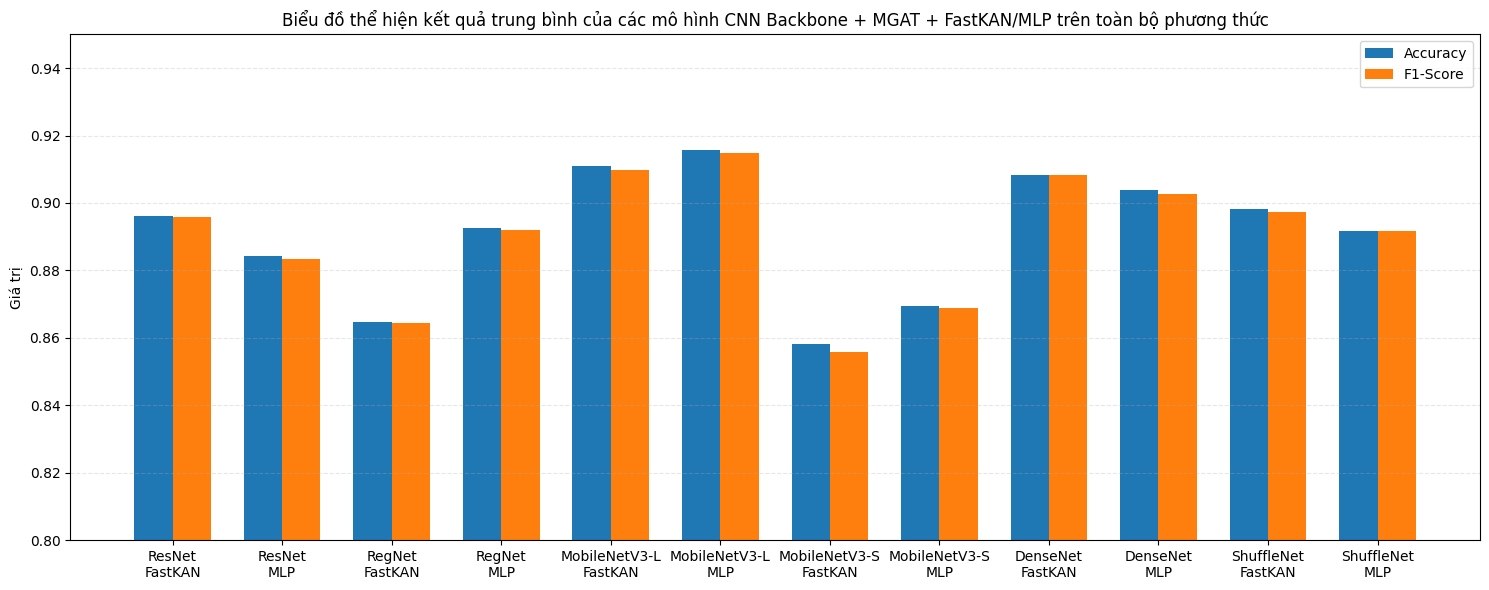
\includegraphics[width=\linewidth]{images/part-02/chap-03/sec-02/PipelineImageText.png}
    \caption{\centering Biểu đồ thể hiện kết quả kiểm thử trung bình của tất cả các mô hình CNN backbone + MGAT + FastKAN/MLP trên hai phương thức}
    \label{fig:KQPipelineImageText}
\end{figure}

\indent Dựa trên bảng tổng hợp và các biểu đồ thể hiện kết quả trung bình của 12 mô hình trên hai phương thức, có thể rút ra các kết luận sau:\vspace{-0.1cm}
\begin{itemize}[label={--}, itemsep=1pt]
    \item Hiệu quả giới hạn của FastKAN trong kịch bản hai phương thức: So với mức cải thiện rõ rệt khi sử dụng đầy đủ ba phương thức (chẳng hạn ResNet18 tăng hơn 3\% so với MLP), thì trong kịch bản chỉ sử dụng hai phương thức, lợi thế của FastKAN thể hiện không rõ ràng, với mức cải thiện chỉ khoảng \textasciitilde 1\%. Điều này cho thấy FastKAN cần một không gian đặc trưng đầu vào đủ phong phú và đa dạng để khai thác hiệu quả khả năng xấp xỉ hàm phi tuyến. Khi thiếu đi thông tin âm thanh, không gian biểu diễn bị thu hẹp, các quan hệ ngữ nghĩa trở nên đơn giản hơn, khiến kiến trúc FastKAN chưa được tận dụng triệt để.

    \item Tính ổn định của MLP trên các backbone MobileNet và RegNet: Với các backbone thuộc dòng MobileNetV3 và RegNetX400MF, MLP cho kết quả ổn định hơn hoặc nhỉnh hơn so với FastKAN. Điển hình là RegNetX400MF, khi kết hợp với MLP đạt độ chính xác 0.8926, cao hơn đáng kể so với 0.8648 của FastKAN. Kết quả này cho thấy đối với dạng đặc trưng được trích xuất từ các backbone này, cấu trúc tuyến tính tương đối đơn giản của MLP phù hợp hơn và ít rủi ro hơn, đồng thời giúp mô hình hội tụ ổn định trong không gian đa phương thức bị rút gọn.
    
    \item Vai trò quan trọng của dữ liệu âm thanh: Mặc dù các mô hình chỉ sử dụng hai phương thức đã cải thiện được kết quả so với CNN Baseline, nhưng khi so sánh với kết quả sử dụng đầy đủ ba phương thức (Mục 2.3), vẫn tồn tại sự chênh lệch đáng kể về độ chính xác (thấp hơn khoảng 2–3\%). Khoảng cách này là minh chứng cho thấy, đối với các bài toán nhận dạng ICH mang tính trình diễn hoặc lễ hội, thông tin từ kênh âm thanh là thành phần quan trọng giúp hoàn thiện biểu diễn ngữ nghĩa và nâng cao hiệu năng tổng thể của hệ thống.
\end{itemize}